
\section{$C^0$ Interior Penalty Method for Biharmonic Equation}
\label{sec:ch1}

\subsection{Introduction of the Boundary Value Problem}%
\label{sub:introduction_of_the_bvp}


In this section do we want to establish a numerical method to fourth order equations. Instead of embarking on the
special case of surface PDE described in \eqref{eq:cahn1} can we establish a general numerical theory on $\mathbb{R} ^2$, which we later can generalize on closed surface later. Assume that we restrict ourself to a compact surface $\Omega \in \mathbb{R} ^2 $ and let $f \in L^{2}\left( \Omega
\right) $ as defined in \ref{sub:l_2_space}.
Let say we want to solve the equation on the form.

\begin{equation}
\label{eq:ch1_bvp}
\begin{split}
    \Delta ^2 u - \beta \Delta u + \gamma u &= f \quad \beta , \gamma \ge 0 \\
    \frac{\partial u}{\partial  n}  &= 0 \quad \text{on }\Omega  \\
    \frac{\partial \Delta u}{\partial  n}  &= q \quad \text{on } \partial \Omega  \\
\end{split}
.\end{equation}

For convenience are the boundary condition $q$ chosen to be defined via a  $\phi \in H^{4}\left( \Omega  \right)$
such that $q = \frac{\partial \Delta \phi }{\partial  n} $ so $\frac{\partial \phi }{\partial  n}  = 0$.
$\partial \Omega $.


\subsection{Weak Formulation}%
\label{sub:weak_formulation}

We want to rewrite \eqref{eq:ch1_bvp} on weak formulation. Now define the Hilbert space \[
V = \left\{ v \in H^2\left( \Omega  \right): \frac{\partial v}{\partial  n}  = 0 \quad \text{on } \partial \Omega
\right\}.
\]
It can be shown \cite{gu2012c0} that a convinient form is to write it as
\begin{equation}
\label{eq:weakform}
    \begin{split}
a\left( u,v \right) &=  \left( f,v \right)_{L^2\left( \Omega  \right)}  - \left( q,v \right)_{L^2\left( \partial \Omega  \right)}  \\
& = \int_{\Omega }^{} D^2 w : D^2 v dx +  \int_{\Omega }^{} \nabla w \nabla v dx + \int_{\Omega }^{} \gamma w \cdot v dx
.\\
    \end{split}
.\end{equation}
For all $\forall v \in  V$, where \[
D^2 w : D^2 v = \sum_{i,j=1}^{2}  \frac{\partial ^2 w}{\partial x_{i} \partial x_{j} } \cdot  \frac{\partial ^2 v
}{\partial x_{i} \partial x_{j} }.
\]

In fact, according to \cite{gu2012c0} can it be shown that the problem has a unique solution if and only if $\gamma >
0$. However, in the case where $\gamma  = 0$ can we provoke a unique solution by introducing the condition \[
\int_{\Omega }^{} f dx = \int_{\partial \Omega }^{}  q ds
\]

Taking this into account can we expand the solution space such that \[
V^* = \begin{cases}
    V, \quad & \text{if } \gamma >0 \\
    \left\{ v \in V: v\left( p^* \right) = 0 \right\}, \quad & \text{if } \gamma  =0
\end{cases}
\]

Where $p^{*}$  is a corner in $\Omega $. In fact, now all solutions of \eqref{eq:weakform} exists in $V^{*}$.


\subsection{Construction of $C^{0}$ Interior Penalty Method}%
\label{sub:construction_interior_penalty_method}

We want to construct a $C^{0}$ interior penalty method based on $C^{0}$ Lagrange elements.
Assume $\mathcal{T}_{h} $ be a triangulation of $\Omega $ and $V_{h}$ be the à $\mathcal{P}_{2} $ Lagrange finite
element space associated with $\mathcal{T}_{h} $ \[
V_{h} = \left\{ v \in C\left( \overline{\Omega } \right) : v_{T} = v |_{T} \in \mathcal{P}_{2}\left( T \right) \quad
\forall T \in  \mathcal{T} _{h}  \right\}
\]
So that we can earn a similar space for the approximated solution space ,
\[
V_{h}^{*} = \begin{cases}
    V_{h}, \quad & \text{for } \gamma >0\\
    \left\{ v \in V_{h}: v\left( p^{*} \right) = 0 \right\} \quad & \text{for } \gamma = 0.
\end{cases}
\]
Here is $p^{*}$ again a corner in $\Omega $. Let us now generalize the Hilbert space as well to the approximated
solution space by defining \[
H^{k}\left( \Omega , \mathcal{T} _{h}  \right) = \left\{ H^{1}\left( \Omega  \right): v_{T} \in H^{k}\left( T
\right)\quad \forall T \in \mathcal{T} _{h} \right\}.
\]
\begin{figure}[!h]
\centering
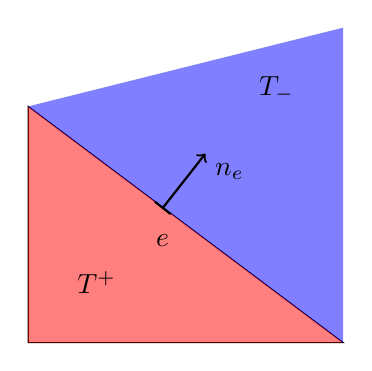
\begin{tikzpicture}[scale=1]
\coordinate (A) at (0,0);
\coordinate (C) at (0,3);
\coordinate (B) at (4,0);
\coordinate (D) at (4,4);
\coordinate (Tm) at (3.5,3.5);
\coordinate (Tp) at (0.5, 0.5);
\coordinate (e) at (1.5, 1.5);
\coordinate (start) at (1.7, 1.7);
\coordinate (end) at (2.25, 2.4);

\draw (A) -- (B) -- (C) -- cycle;
\fill[red, opacity=0.5] (A) -- (B) -- (C);
\fill[blue, opacity=0.5] (B) -- (C) -- (D);
\node[below left] at (Tm) {$T_{-} $ };
\node[above right] at (Tp) {$T^{+}$ };
\node[below right] at (e) {$e$ };

\draw [|->, thick] (start) -- (end);
% \node[above right] at (A) {A };
% \node[below right] at (B) {B};
% \node[above right] at (C) {C };
% \node[below right] at (D) {D};
\node[below right] at (end) {$n_e$};
\end{tikzpicture}
\caption{Edge $e$ shared by the triangles $T_{-}$ and $T_{+}$ and the normal unit vector $n_{e}$.  }
    \label{fig:normal}
\end{figure}

Now assume that that $e \in \mathcal{E}_{h}^{i} $ is shared between two triangles $T_{-}, T_{+} \in  \mathcal{T} _{h}$ .
Then we can assume that the unit normal from $T_{-}$ to $T_{+}$ is described as $n_{e}$ as illustrated in figure
\ref{fig:normal}. Finally, we now want to define jumps internally, \[
\begin{split}
    \jump{ \frac{\partial v_{h}}{\partial n_{e}} } &= \frac{\partial v_{T_{+}}}{\partial n_{e}  } | _{e} -
    \frac{\partial v_{T_{-}}}{\partial n_{e}  } |_{e}, \quad \forall v \in H^{2}\left( \Omega , \mathcal{T} _{h} \right)  \\
    \jump{ \frac{\partial ^2 v_{h}}{\partial n_{e} ^2 } } &= \frac{\partial ^2 v_{T_{+}}}{\partial  n_{e}^2} |_{e}  -
    \frac{\partial ^2 v_{T_{-}}}{\partial n_{e}^2   } |_{e} \quad \forall v \in H^3\left( \Omega , \mathcal{T} _{h}
    \right).  \\
\end{split}
\]

And similarly for means internally,
\[
    \begin{split}
\mean{ \frac{\partial v_{T_{-}}}{\partial n_{e} } } &= \frac{1}{2} \left( \frac{\partial v_{T_{+}}}{\partial n_{e} }
|_{e} +  \frac{\partial v_{T_{-}}}{\partial n_{e} } |_{e}  \right) \quad  \forall v \in H^2\left( \Omega , \mathcal{T}
_{h} \right) \\
    \mean{ \frac{\partial ^2 v_{h}}{\partial n_{e}^2 } } &= \frac{1}{2} \left( \frac{\partial ^2 v_{T_{+}}}{\partial
    n_{e}^2  } |_{e} + \frac{\partial ^2 v_{T_{-}}}{\partial n_{e}^2  } |_{e}    \right) \quad \forall v \in  H^3\left( \Omega .
\mathcal{T}_{h}  \right), \\
    \end{split}
\]

Let the edges along the boundary be defined as $e \in  \mathcal{E} _{h}^{b}$ along a some boundary triangle $\mathcal{T}
_{h}$. We can then define the jump and mean as \[
\begin{split}
    \jump{ \frac{\partial v_{h} }{\partial n_{e} } } & = -\frac{\partial v_{T}}{\partial  n_{e}} |_{e} \quad \forall v \in
    H^2\left( \Omega , \mathcal{T}_{h}  \right) \\
    \mean{ \frac{\partial ^2 v_{h}}{\partial n_{e}^2 } } & = \frac{\partial v_{T}}{\partial  n_{e}} |_{e} \quad \forall v \in
    H^3\left( \Omega  , \mathcal{T}_{h}  \right)
\end{split}
\]

Using the results from \cite{gu2012c0} can we formulate the discrete formulation the boundary value problem
\eqref{eq:ch1_bvp} using $C^{0}$ interior penalty method. Our goals is to find a $u_{h} \in V_{h}^{*} $ such that this
is true,

\begin{equation}
\label{eq:C0-methoda}
\mathcal{A} \left( u_{h}, v_{h}  \right) = \left( f, v_{h} \right)_{L^{2}\left( \Omega  \right)} - \left( q, v_{h}
\right) _{L^{2}\left( \partial \Omega  \right)} \quad  \forall v_{h} \in V_{h}^{*}
.\end{equation}

Where $w_{h}, v_{h} \in  V_{h}$ and
\begin{equation}
\label{eq:C0-methodb}
\begin{split}
    \mathcal{A} \left( w_{h}, v_{h} \right) &=  \sum_{T \in \mathcal{T} _{h}}^{} \int_{T}^{} D^2 w_{h} : D^2 v_{h}  \\
    & + \sum_{e \in  \mathcal{E} _{h}}^{} \int_{e}^{ } \mean{ \frac{\partial ^2 w _{h}}{\partial n_{e}^2 } } \jump{
    \frac{\partial v_{h}}{\partial  n_{e}} }  ds \\
    & + \sum_{e \in \mathcal{E} _{h}}^{} \mean{ \frac{\partial ^2
v_{h}}{\partial n_{e }^2 } } \jump{ \frac{\partial w_{h}}{\partial n_{e}} }  ds \\
 &  + \sum_{e \in \mathcal{E} _{h}}^{} \frac{\sigma }{\left\lvert e \right\rvert } \int_{e}^{} \jump{ \frac{\partial
 w_{h}}{\partial n_{e}}} \jump{ \frac{\partial v_{h}}{\partial n_{e}} } ds \\
 & + \int_{\Omega }^{}  \beta \nabla w_{h} \cdot \nabla v_{h} dx + \int_{\Omega }^{} \gamma w_{h} v_{h} dx .
\end{split}
.\end{equation}

The notation $\left\lvert e \right\rvert $ is to describe the length of the edge $e$ and $\sigma  \ge  1$ is a penalty
parameter.




\subsection{Hybrid DG Biharmonic Equation}%
\label{sub:hybrid_dg_biharmonic_equation}

Let us again define the problem

\begin{equation}
\label{eq:HDG_bi_problem}
\begin{split}
    \nabla ^4 u & = f \quad \text{in } \Omega   \\
    \partial _{n} u & = \partial _{n} \nabla ^2 u = 0 \quad \text{on } \partial \Omega   \\
\end{split}
.\end{equation}

In fact, we must also assume the solvability condtion $ \int_{\Omega }^{} f dx = 0$ to obtain a unique solution according to
equation (2.4) in Brenner \cite{brenner2012}, which also can be related to equation (3.4) in Gu \cite{gu2012c0}.

Anyhow,
let us first define the Hilbert space of the discrete solution \[
\begin{split}
    H^{1}\left( \mathcal{T}_{h}  \right)  & = \left\{ v \in L_{2} \left( \Omega  \right) : v  \mid _{T} \in H^{1} \left( T
    \right) \forall T \in \mathcal{T}_{h}    \right\} \\
    V &=  \left\{ v \in H^2\left( \Omega  \right) : \partial _{n} v = 0 \text{ and } \partial _{n} \nabla ^2 v = 0 \text{ on } \partial \Omega  \right\} \\
\end{split}
\]
\todo[inline]{ Probably need to work more on this argumentation }

Let us now define $u,v \in V$.

\subsubsection{HDG Method}%
\label{ssub:dg_method}
Let us now define our workspace using the Hilbert spaces
 \[
\begin{split}
    V &=  \left\{ \left( u, u_{F}  \right): u \in H^{4}\left( \mathcal{T} _{h} \right) \cap H^{1}\left( \Omega  \right)   \right\} \\
    V_{h} &=  \left\{ \left( u, u_{F}  \right) : u \in \mathcal{P} ^{k}\left( T \right) \forall T \in  \mathcal{T} ,
    u_{F} \in \mathcal{P} ^{k}\left( E \right) \in  \mathcal{F}_{h}    \right\} \\
\end{split}
\]

and the ones including the null drichlet conditions \[
\begin{split}
    V_{0} &= \left\{ \left( u, u_{F} \right) \in  V : \quad u =0, u_{F} = 0 \text{ on } \partial \Omega   \right\}, \\
    V_{0,h} &= \left\{ \left( u, u_{F} \right) \in  V_{h} : \quad u =0, u_{F} = 0 \text{ on } \partial \Omega   \right\}
   . \\
\end{split}
\]
Let $\left( u, u_{F} \right) \in  V $\[
    \begin{split}
\sum_{T}^{} \left( \nabla ^{4} u,v \right) & = \sum_{T}^{} \left( \nabla ^{3} u, \nabla  v \right)_{T} + \left<\partial _{n}
\nabla ^2 u, v \right>_{\partial \Omega } \\
&= \sum_{T}^{} \left( \nabla ^2 u, \nabla ^2 v \right)_{T} - \left<\partial _{n} \nabla u, \nabla v \right>_{\partial T}
+ \left< \partial _{n} \nabla ^2 u, v \right> _{\partial T}\\
    \end{split}
\]


\subsubsection{Basic DG method}%
\label{ssub:basic_dg_method}
Let $w,v \in  H^{4} \left( T  \right) $. Using the same method as in equation (3.6) in  \cite{gu2012c0} can we
deduce that for every triangle $T \in  \mathcal{F}_{h} $ \[
    \begin{split}
        \left( \nabla ^{4} w, v \right) _{T} &= \left< \partial _{n} \nabla ^2 w, v \right>_{\partial T} - \left( \nabla \left( \nabla ^2 w
 \right), \nabla  v  \right)_{T}   \\
 &= \left( D^2w, D^2v \right)_{T} + \left< \partial _{n} \nabla ^2 w, v \right>_{\partial T}  - \left<\partial _{n}
 \nabla w, \nabla v \right>_{\partial T} \\
 &=  \left( D^2 w, D^2 v \right)_{T} - \left<\partial _{nt} w, \partial _{t} v \right>_{\partial T} - \left<\partial
 _{nn} w, \partial _{n} v \right> _{\partial T} +  \left<\partial _{n} \nabla ^2 w, v \right> \\
    \end{split}
\]
Keep in mind that this is a results by defining $\nabla  = \left( \partial _{n}, \partial _{t} \right) $ such that
$\left<\partial _{n} \nabla w, \nabla v \right>_{\partial T} = \left<\partial _{nt} w, \partial _{t} v\right> _{\partial
T} + \left< \partial _{nn} w, \partial _{n} v  \right> _{\partial T} $. Thus, letting $u,v \in
H^{4}\left( T  \right) $  does this hold for local continuity

\begin{equation}
\label{eq:bi_basic_dg}
\left( \nabla ^{4} u,v \right) _{T} = \left( D^2u,D^2v \right) _{T } - \left<\partial _{nt} u, \partial _{t}v
\right>_{\partial t} - \left<\partial _{nn} u, \partial _{n}v \right>_{\partial T} + \left<\partial _{n} \nabla ^2 u,v
\right>_{\partial T}
.\end{equation}

For global continuity  it ends up with

\begin{equation}
\label{eq:bi_basic_dg_full_1}
\left( \nabla ^{4} u, v \right) _{\Omega }
= \sum_{T \in  \mathcal{T} _{h}}^{} \left( D^2u, D^2v \right)_{T}  + \sum_{E \in
\mathcal{F} ^{ext}_{}}^{} \left<\partial _{n} \nabla  ^2 u, v  \right> _{E}
- \left<\partial _{nt} u, \partial _{n} v \right> _{E}
+ \sum_{E \in \mathcal{F}  ^{int}}^{} \left<\partial _{nn} u , \jump{ \partial _{n_{e}} v }
\right>_{E}
.\end{equation}

What we see is that for \eqref{eq:bi_basic_dg} and \eqref{eq:bi_basic_dg_full_1} to be equivalent on normal and global form must this be true
\[
 \sum_{T \in  \mathcal{T}_{h} }^{}  - \left<\partial _{nt} u, \partial _{t}v
\right>_{\partial T} - \left<\partial _{nn} u, \partial _{n}v \right>_{\partial T} + \left<\partial _{n} \nabla ^2 u,v
\right>_{\partial T}
=  \sum_{E \in
\mathcal{F}^{ext}  }^{} \left<\partial _{n} \nabla  ^2 u, v  \right> _{E}
- \left<\partial _{nt} u, \partial _{n} v \right> _{E}
+ \sum_{E \in \mathcal{F}^{int} }^{} \left<\partial _{nn} u , \jump{ \partial _{n_{e}} v }
\right>_{E}
\]

Anyhow, \textbf{assuming} that this equation holds can we introduce following terms,  \[
    \begin{split}
    &  \left< \partial _{n} v  , \jump{ u }\right> _{\partial T} \text{ for symmetry} \\
    & \tau_{h} \left<\jump{ u }, \jump{ v }\right> _{\partial T} \text{ for stability} \\
    \end{split}
\]

\todo[inline]{ Might want to rethink the notation of $n_{e}$  }
Keep in mind that the jump is defined as $\jump{ \partial _{ne} v } = n_{e} \left( \nabla v_{+} - \nabla v_{-} \right)   $
and we have now the basic DG method

\begin{equation}
\label{eq:bi_basic_dg_full}
\begin{split}
\left( \nabla ^{4} u, v \right) _{\Omega }
= & \sum_{T \in  \mathcal{T} _{h}}^{} \left( D^2u, D^2v \right)_{T}  + \sum_{E \in
\mathcal{F} ^{ext}_{}}^{} \left<\partial _{n} \nabla  ^2 u, v  \right> _{E}
- \left<\partial _{nt} u, \partial _{n} v \right> _{E}
+ \sum_{E \in \mathcal{F}  ^{int}}^{} \left<\partial _{nn} u , \jump{ \partial _{n_{e}} v }
\right>_{E} \\
 & + \left< \partial _{n} v  , \jump{ u }\right> _{\partial T} +
\tau_{h} \left<\jump{ u }, \jump{ v }\right> _{\partial T}
\end{split}
.\end{equation}

\subsubsection{HC0IP Method copied from NGSolve}%
\label{ssub:hc0ip_method_from_ngsolve}


We consider the Kirchhoff plate equation: Find $w \in H^2$, such that
$$
\int \nabla^2 w : \nabla^2 v = \int f v
$$

A conforming method requires $C^1$ continuous finite elements. But there is no good option available, and thus there is no $H^2$ conforming finite element space in NGSolve.

$$
\sum_T \nabla^2 w : \nabla^2 v
- \int_{E} \{\nabla^2 w\}_{nn} \, [\partial_n v]
- \int_{E} \{\nabla^2 v\}_{nn} \, [\partial_n w] + \alpha \int_E  [\partial_n w]  [\partial_n v]
$$

[Baker 77, Brenner Gudi Sung, 2010]

We consider its hybrid DG version, where the normal derivative is a new, facet-based variable:

$$
\sum_T \nabla^2 w : \nabla^2 v
- \int_{\partial T} (\nabla^2 w)_{nn} \, (\partial_n v - \widehat{v_n})
- \int_{\partial T} (\nabla^2 v)_{nn} \, (\partial_n w - \widehat{w_n}) + \alpha \int_E (\partial_n v - \widehat{v_n}) (\partial_n w - \widehat{w_n})
$$










